\mytitlepage{Прикладной математики}{1}{Комьютерная графика}{Введение в программирование с использованием OpenGL}{ПМ-63}{Шепрут И.И.}{9}{Задорожный А.Г.}{2019}

\section{Цель работы}

Ознакомиться с основами использования библиотеки OpenGL и работе с примитивами.

\section{Постановка задачи}

\noindent\normalsize{\begin{easylist}
\ListProperties(Hang1=true)
& Отобразить в окне множество примитивов (вершины которых задаются кликами мыши) в соответствии с вариантом задания.
& Для завершения текущего (активного) набора (множества) примитивов и начала нового зарезервировать специальную клавишу (пробел или правый клик).
& Для текущего набора примитивов предоставить возможность изменения цвета и координат его вершин.
& Текущее множество примитивов выделять среди других, например, изменением размера его вершин командой \texttt{glPointSize(*)}.
& Использовать контейнер \texttt{vector} из библиотеки \texttt{STL} для хранения набора примитивов и множества вершин каждого примитива, а для хранения атрибутов рекомендуется использовать стандартный класс \texttt{struct}. 
& Предусмотреть возможность удаления последнего примитива и последнего набора примитивов.
& Продублировать команды в меню, созданном с помощью библиотеки \texttt{GLUT}.
\end{easylist}}

Вариант: \mycodeinline{c++}{9. GL_QUAD_STRIP}.

\section{Реализованные функции}

\noindent\normalsize{\begin{easylist}
\ListProperties(Hide=100, Hang1=true, 
	Progressive*=.5cm,%	
	Style1*=\textbullet ,%
	Style2*=\textopenbullet )
& \textbf{Выделение произвольного примитива как текущий с помощью мыши.}
& Добавление, удаление примитива.
& Операции над текущим примитивом:
&& Добавление, удаление точки.
&& \textbf{Изменение координаты произвольной точки с помощью мыши.}
&& Изменение цвета примитива (в том числе и альфа-канала).
&& Масштабирование примитива.
&& \textbf{Вращение примитива вокруг мыши.}
& Все функции продублированы в меню, там же написана клавиша, реализующая эту функцию.
& При рисовании используется двойная буферизация.
\end{easylist}}

\section{Пример реализованных функций}

\subsection{Меню}

В меню так же с отступом написано как воспользоваться данной возможностью при помощи клавиатуры, а конкретно, там сказана клавиша, реализующая это действие. Так же там говорится какие действия выполняются с помощью мыши и колесика мыши.

\begin{center}
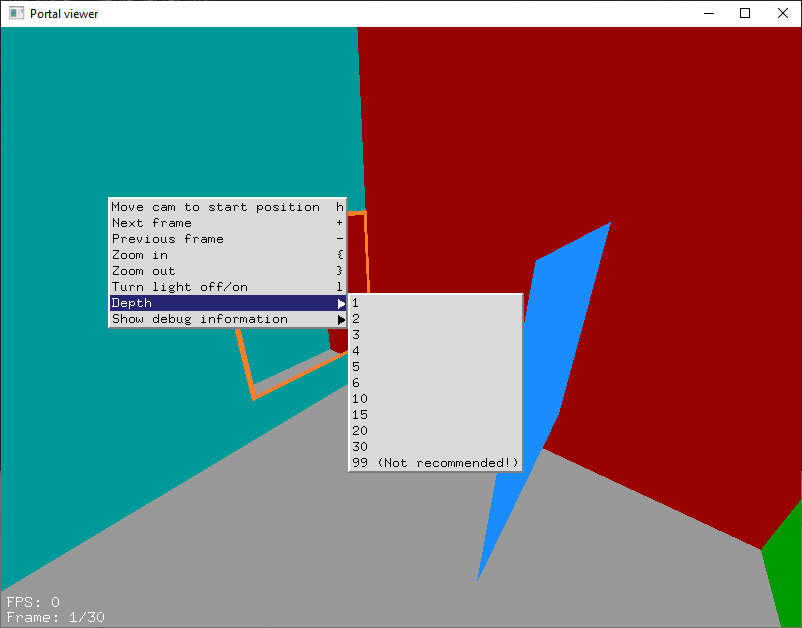
\includegraphics[scale=0.75]{1.png}
\end{center}

\subsection{Выбор произвольного примитива с помощью мыши}

\begin{center}
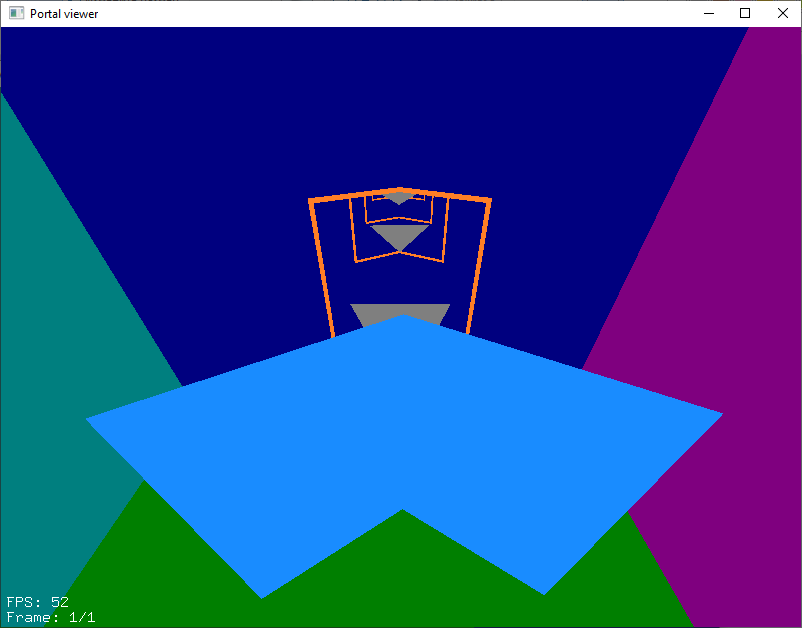
\includegraphics[width=.48\textwidth]{9.png}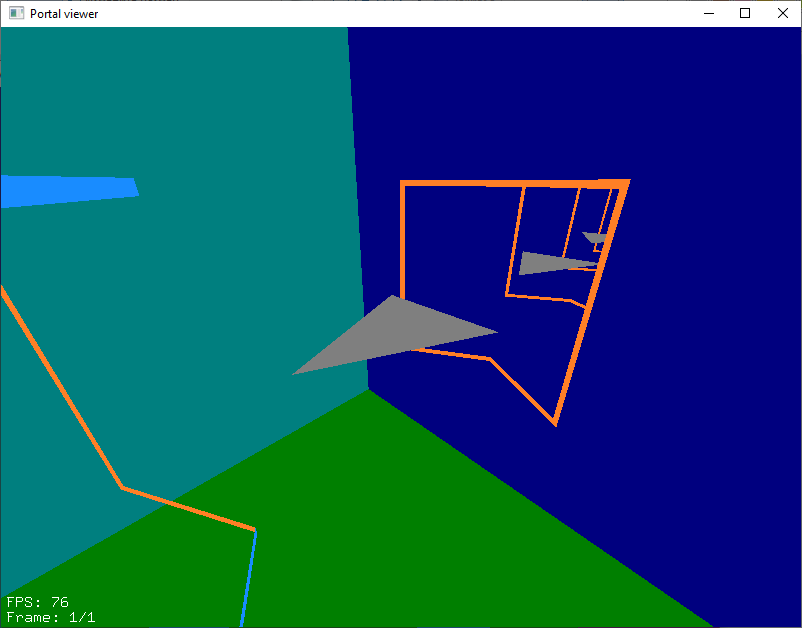
\includegraphics[width=.48\textwidth]{10.png}
\end{center}

\subsection{Перемещение примитива}

\begin{center}
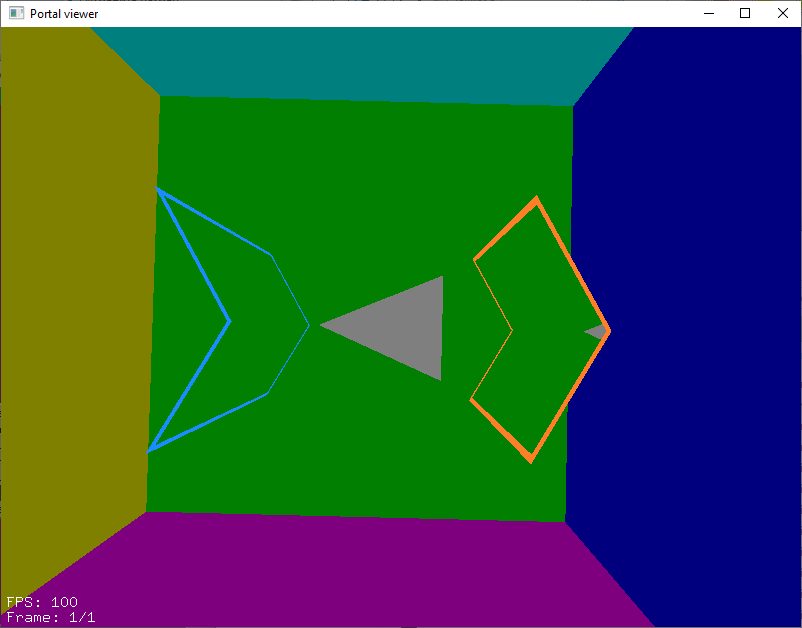
\includegraphics[width=.48\textwidth]{7.png}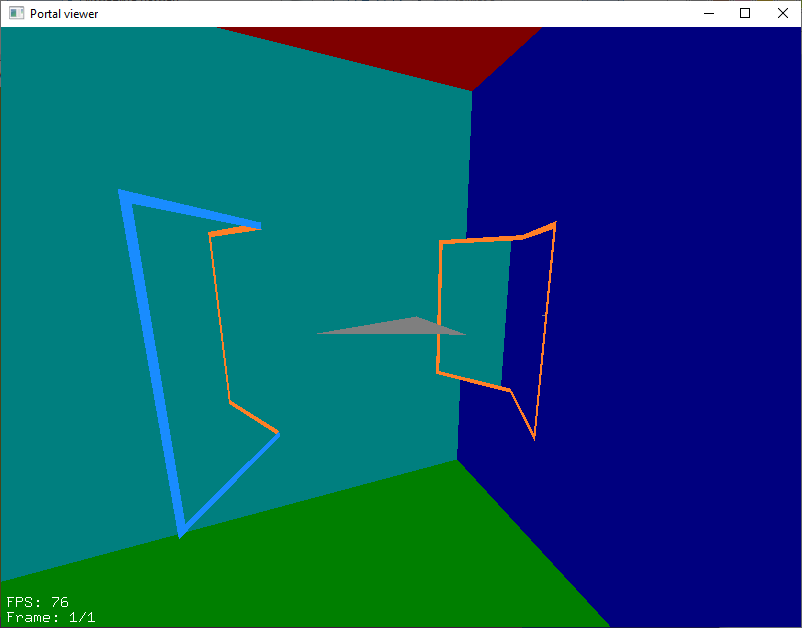
\includegraphics[width=.48\textwidth]{8.png}
\end{center}

\subsection{Масштабирование примитива}

\begin{center}
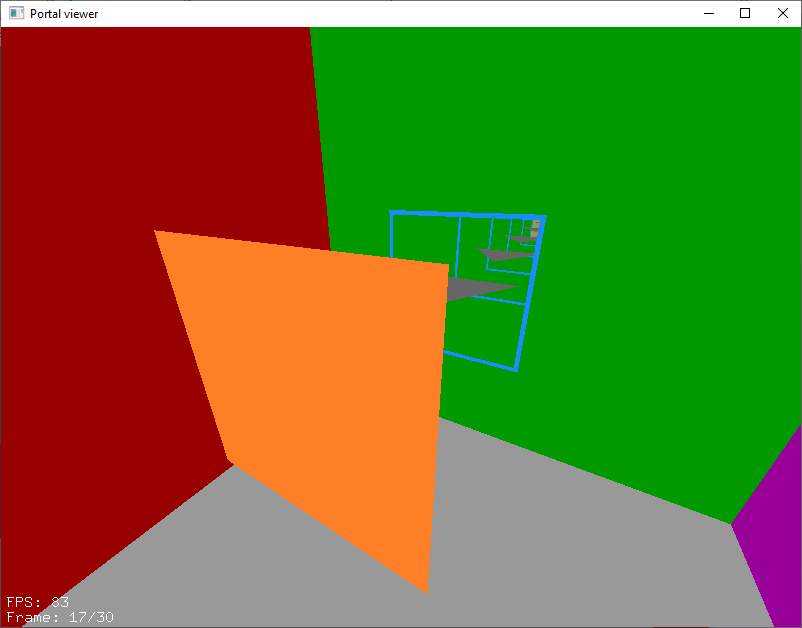
\includegraphics[width=.48\textwidth]{5.png}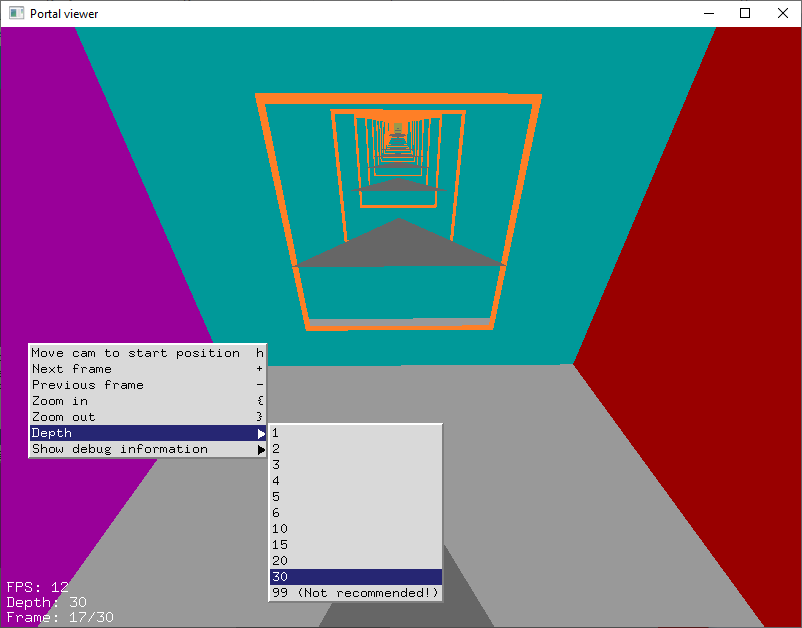
\includegraphics[width=.48\textwidth]{6.png}
\end{center}

\subsection{Вращение текущего примитива вокруг мыши}

\begin{center}
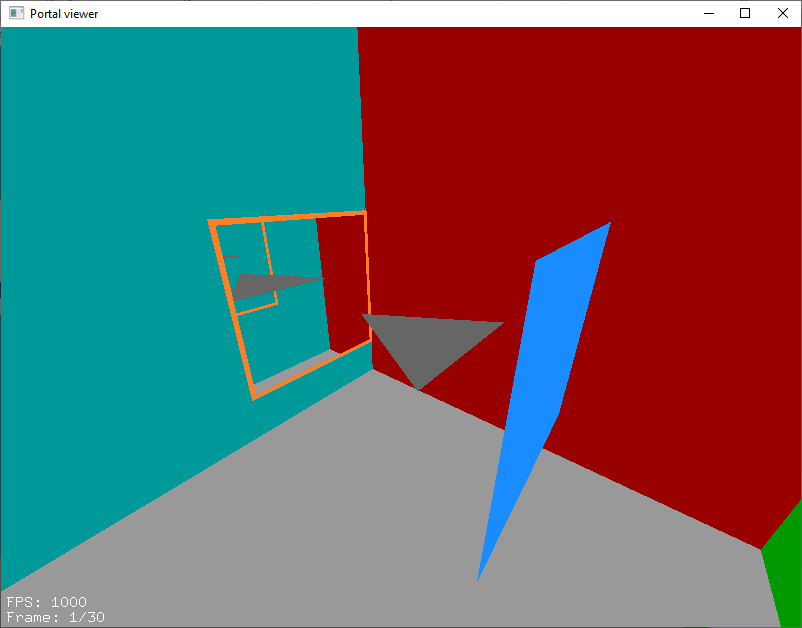
\includegraphics[width=.48\textwidth]{2.png}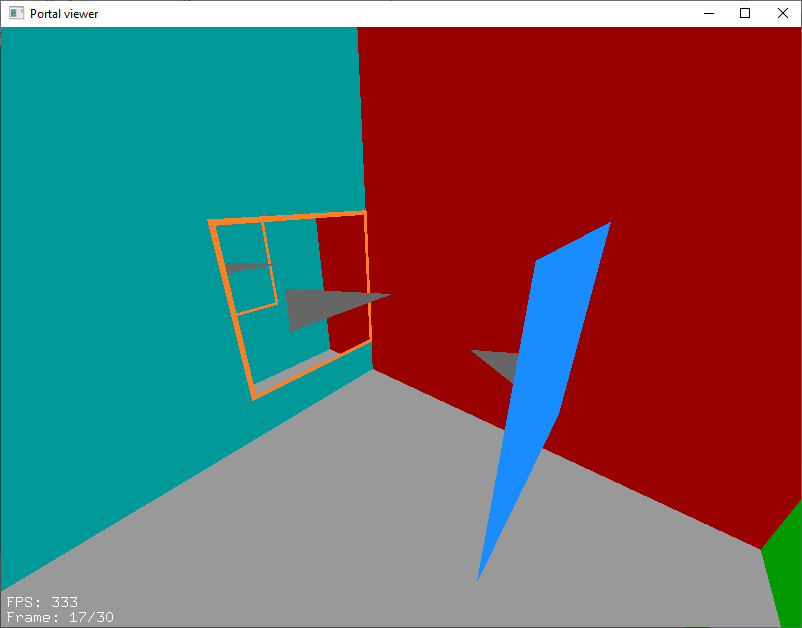
\includegraphics[width=.48\textwidth]{3.png}
\end{center}

\subsection{Изменение произвольной точки примитива}

\begin{center}
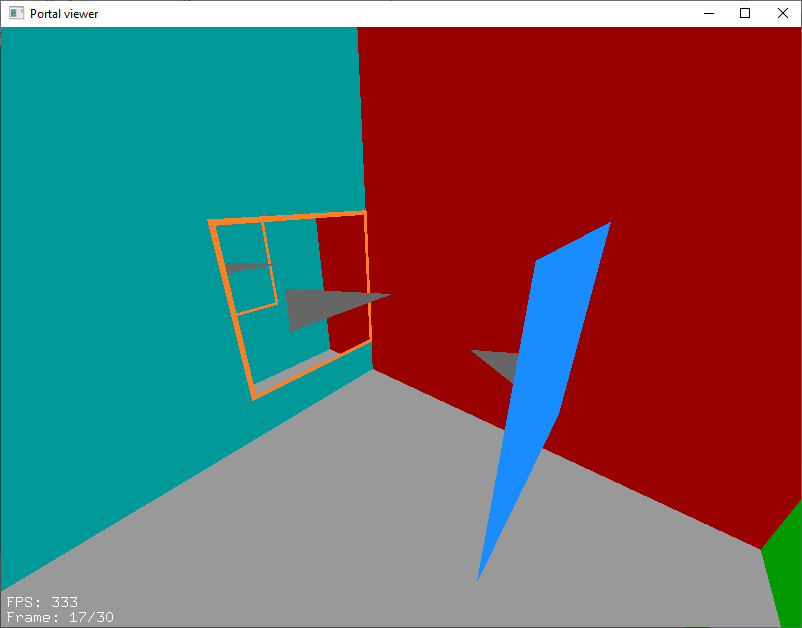
\includegraphics[width=.48\textwidth]{3.png}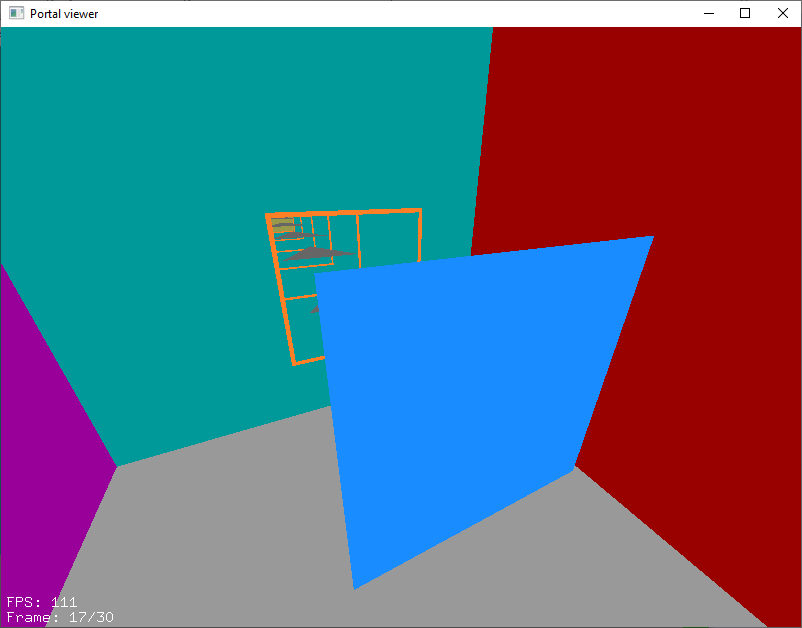
\includegraphics[width=.48\textwidth]{4.png}
\end{center}

\section{Код программы}

\mycodeinput{c++}{../main.cpp}{main.cpp}
\mycodeinput{c++}{../interface.h}{interface.h}
\mycodeinput{c++}{../interface.cpp}{interface.cpp}